%!TEX root = ../template.tex
%%%%%%%%%%%%%%%%%%%%%%%%%%%%%%%%%%%%%%%%%%%%%%%%%%%%%%%%%%%%%%%%%%%%
%% chapter2.tex
%% NOVA thesis document file
%%
%% Chapter with the template manual
%%%%%%%%%%%%%%%%%%%%%%%%%%%%%%%%%%%%%%%%%%%%%%%%%%%%%%%%%%%%%%%%%%%%
\chapter{Related Work}
\label{cha:related_work}
Since the users are a fundamental component on the study, their relationship with data and what are their expectations to these query systems will be discussed. Moreover, a set of technologies and techniques will be described and compared. This information can turn to be useful to explore solutions, and understand different points of view to manage problems, regarding the project scope. As the project is focused on the improvement of an interface that combines the query design with the query output viewer. 

\section{Query Conceptual Models}
\label{sec:query_conceptual_models}
The perception of the user's conceptual model is important to understand how the user reason while interacting with the system the perform the intended actions. A query is built with the aim of gathering data. To transmit what is the intended data, the user needs to think about how it could express the data required in the query.

%The understanding of the user's conceptual model leads to remove the existing gap between what the user wants to query from the database and what system register that the user wants to retrieve.

Some studies have analyzed this reasoning process of the users when was writing queries. Siau \textit{et al.} \cite{effectsOfQueryComplexityAndLearningOnNoviceUserQueryPerformance} have referred that "The semantics communicated through the interface can be classified according to abstraction levels, such as the conceptual and logical levels". Considering a physical level, an interface that involves system details, such as physical storage and access structures, and a logical level that takes into account abstract structures for data and operations. Through an empirical method of evaluation, the conceptual level has revealed a higher accuracy. Also, this abstraction level makes the users more confident in their answers than the physical level or logical levels. Moreover, the time that users need to design the queries is reduced using conceptual levels. \cite{effectsOfQueryComplexityAndLearningOnNoviceUserQueryPerformance}

Reisner \cite{humanFactorStudiesOfDatabaseQueryLanguages} provided a model of query writing from the reading of the query intention in an English statement to the query writing in SQL (Figure \ref{fig:reisner_model}). After understanding what data is required, the user applies two parallel steps. In the \textbf{Template Generation} phase, the user formulates a template identifying the SQL keywords necessary, such as SELECT, FROM, and WHERE. In the other step, called \textbf{Lexical Transformation}, the user identifies the name of the tables and columns involved. Finally, the results of these two steps are combined in the last step, denominated \textbf{Insertion}, in order to produce the final query \cite{humanFactorStudiesOfDatabaseQueryLanguages}. The recall of table and column names represents a significant use of long-term memory, being a concern that should be taken into account \cite{userErrorsInDatabaseQueryComposition}.

In the same field, Odgen \cite{implicationsOfACognitiveModelOfDatabaseQuery} presented a three-stage cognitive model of the query process (Figure \ref{fig:odgen_model}):

\begin{enumerate}
  \item \textbf{Query Formulation}: according to the existing data, the user specifies, in natural language, what data is required;
  \item \textbf{Query Translation}: regarding the existing data model, the operations and relations necessary are defined, in order to adapt the natural language request to the pragmatics of the intended query;
  \item \textbf{Query Writing}: the information of the previous steps is used to built the query, using the syntactic and the semantics of the query language.
\end{enumerate}

Comparing the two previous models presented, the Lexical Transformation phase is present in the Query Translation phase of the latter model, as well as, Template Generation and insertion are part of the Query Writing phase. \cite{anEvaluationOfNoviceEndUserComputingPerformance} Moreover, although the query writing and comprehension are the focus of this work, it was verified in a comparison between three different models (relational model, extended-entity-relationship model, and object-oriented model) that the data model influence the query writing and comprehension. \cite{anEvaluationOfNoviceEndUserComputingPerformance}

\begin{figure}[htbp]
  \centering
  \subcaptionbox{Reisner Model\label{fig:reisner_model}} %
    {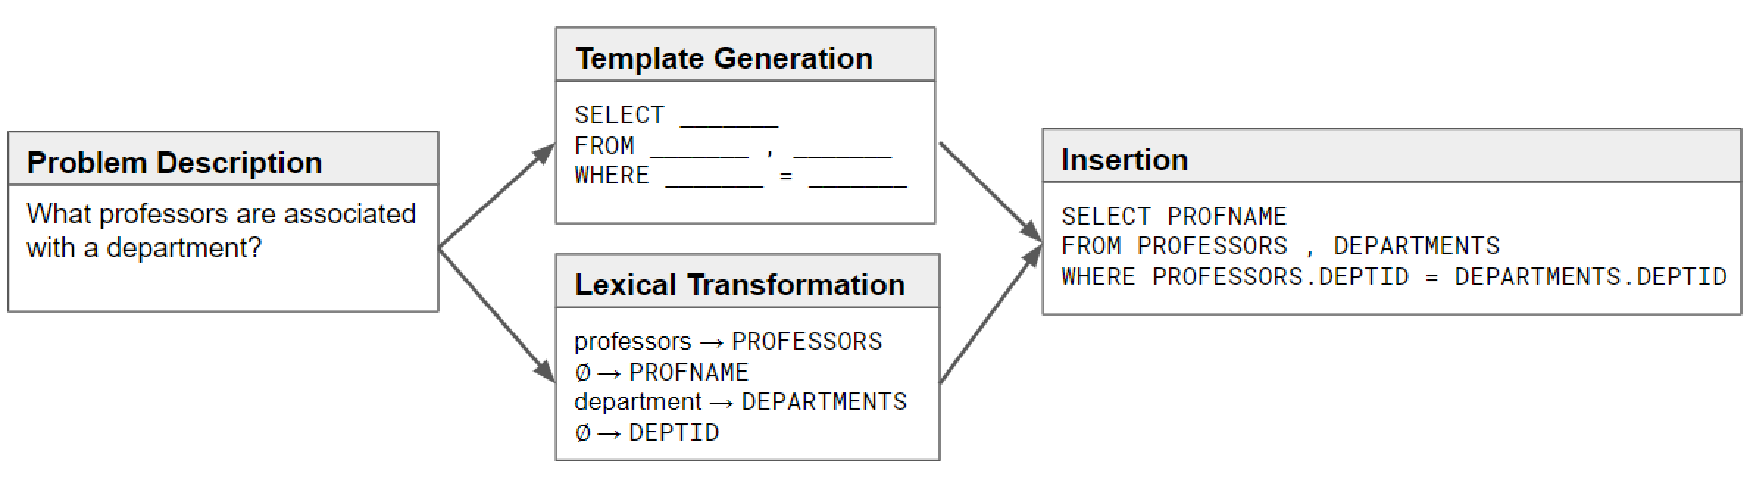
\includegraphics[width=0.5\linewidth]{reisner-model}}%
  \subcaptionbox{Odgen Model \label{fig:odgen_model} }%
    {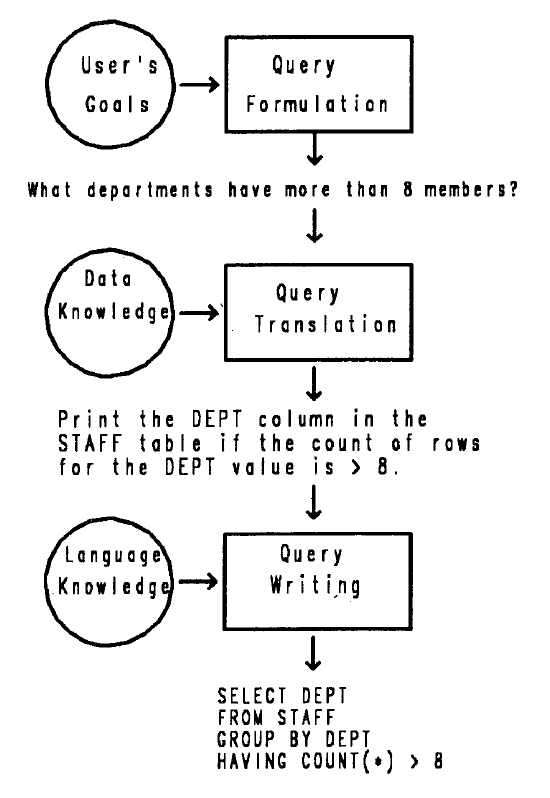
\includegraphics[width=0.5\linewidth]{odgen-model}}%
\caption{Models of Query Writing Process.}
  \label{fig:models_of_query_writing_process}
\end{figure}

The query comprehension is one of the important concerns of this work, since it is important to consider if the query representation, no matter if it is visual or textual, indicates clearly what data will be gathering. %TODO: pode ser importante dar exemplos da importancia da comprehension (e.g., para quem vai ler; se o escritor foi diferente do leitor, etc.) 
Chan \textit{et al.} \cite{anEvaluationOfNoviceEndUserComputingPerformance} have postulated that the query comprehension could be covered by the reverse of the stages included in the Odgen Model. First, the user should identify the data structure and operations, to translate them, in the next step, to the natural language. After this, the user needs to read and understand what data gathering is intended. Moreover, in this evaluation, it was concluded that although data modeling influence query writing, it does not influence the query comprehension. The explanation is provided by the authors: "Both query writing and comprehension require understanding of the query language syntax. This is a component not needed in the data modeling task."

The experience with the data involved is another factor that influences the query comprehension. If novice users do not understand the data involved, they cannot validate if the query result is correct. This situation was analyzed by Robb \textit{et al.} that were distinguished the query process between new users and experienced users (Figure \ref{fig:ex_ante_expectations}). Besides, they were concluded that if the novice users were alerted to the details of the data queried, the query effectiveness will increase.

\begin{figure}[htbp]
  \centering
    {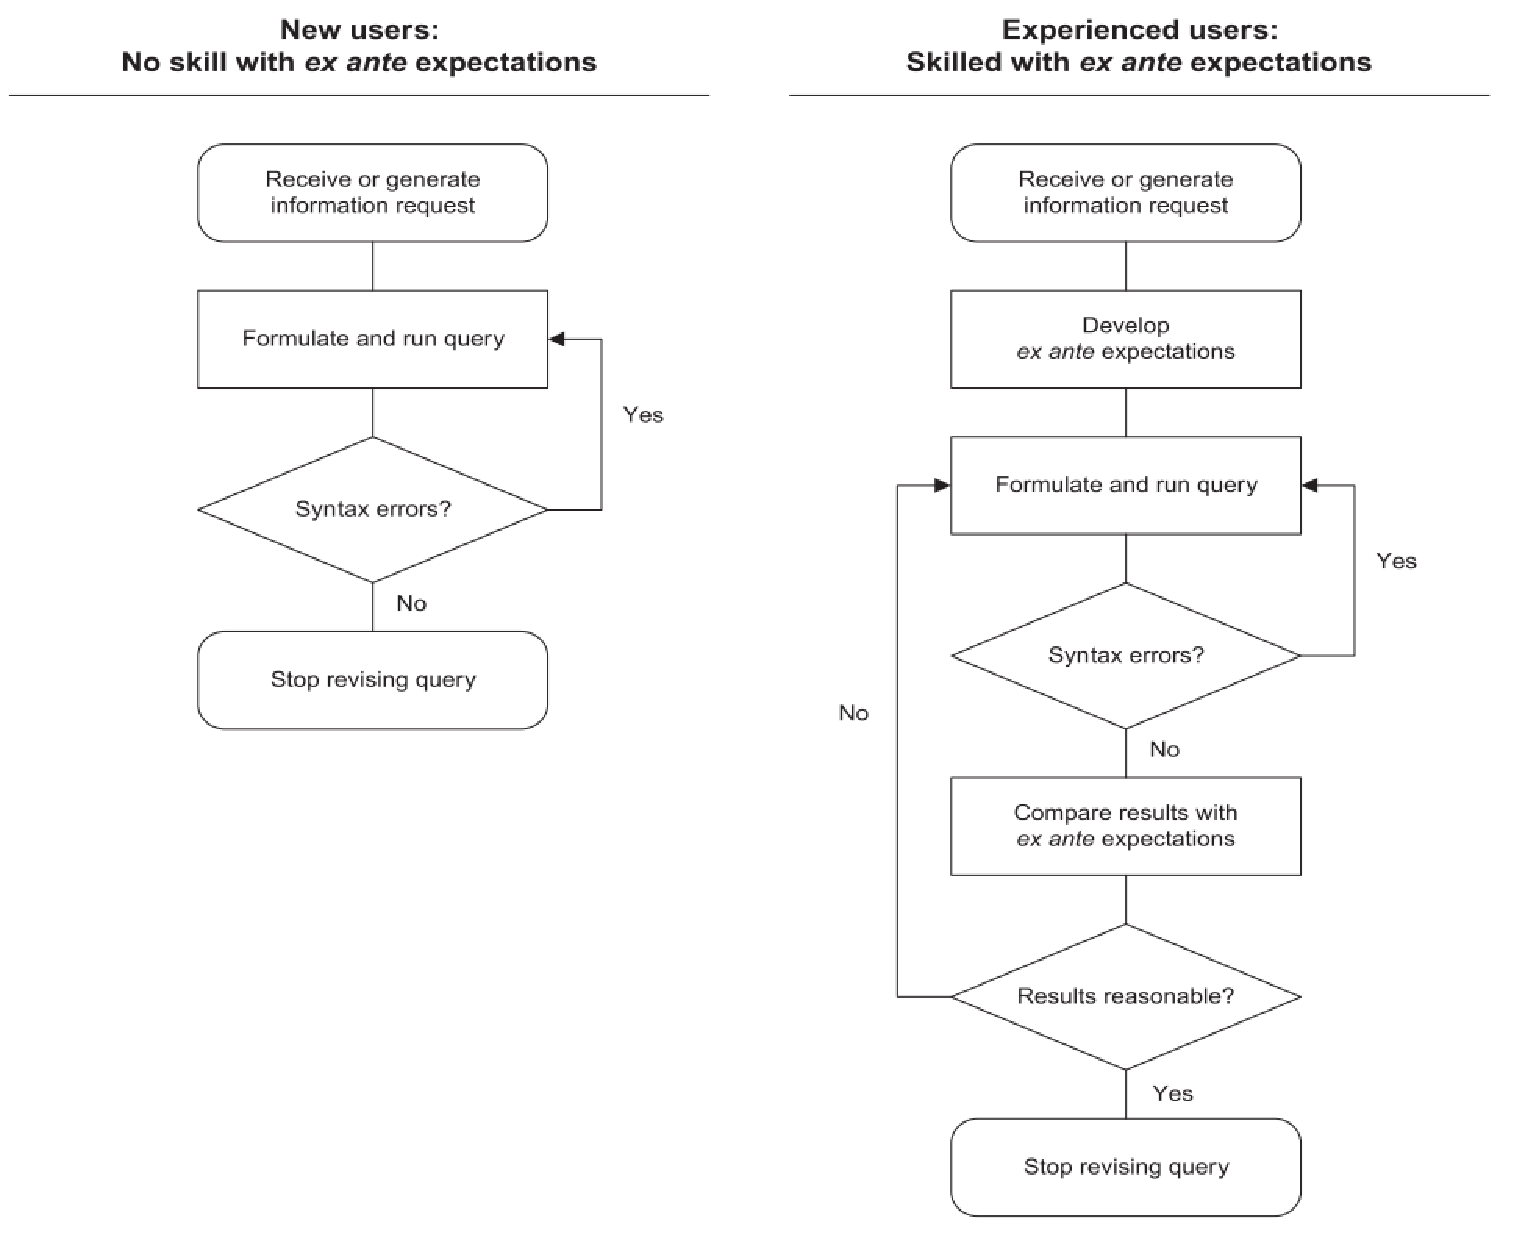
\includegraphics[width=0.9\linewidth]{ex-ante-expectations}}%
\caption{New and experienced users’ query processes (extracted from \cite{improvingNewUsersQueryPerformance}).}
  \label{fig:ex_ante_expectations}
\end{figure}


\section{Query Formulation Problems}
\label{sec:query_formulation_problems}
Since the goal of this work is the improvement of an interface that allows its user to build queries, it is important to summarize what are the problems that usually occur in query formulation. The problems that will be presented are related to SQL queries. However, as the visual tool of this work aims to substitute some functionalities of SQL, the comprehension of the interaction problems that exist in the textual language can be considered and mitigated in the development of the new interface. 

The query errors could be syntactic or semantic. The syntactic errors are related to the grammar rules of the language and are detected by the compiler. Therefore, the impact of these errors is reduced since the user can see that the query is incorrect through the compiler alert. The semantic errors are a major concern because they occur when the returned information is not the intended by the user, even if the query does not have compilation errors. \cite{userErrorsInDatabaseQueryComposition} These errors could affect the correctness of the results.

The most relevant semantic problems are related with boolean operators of the query and with joins omission.

%\section{Low-code Development Users}
%\label{sec:low_code_development_users}

\section{Visual Query Composition}
\label{sec:visual_query_composition}

The interfaces to build queries resort on visual representations to communicate with the user. Catarci \textit{et al.} \cite{visualQuerySystemsForDatabases_aSurvey} presented an interesting classification according to the visual formalism which the interface is based on:

\begin{itemize}
    \item \textbf{Form-based}: based on forms, which can be seen as a rectangular grid of other components (subforms, groups of cells, a combination of cells, etc.) that group objects in a named collection regarding its structure. Forms and tables are similar,  but contrary to the tables, forms allow nesting. Thus, forms can be seen as a generalization of tables. In this approach, the relationships can be represented among cells, cells subsets, or even the overall set, providing to the user three information levels; %TODO: example of QBE 
    \item \textbf{Diagram-based}: usage of graphical representations, such as graphs, charts, and diagrams to better transmit the relationships among data. The aim is to use visual representations to help the understanding of the relationships between concepts which are represented by textual labels;
    \item \textbf{Icon-based}: as the opposite of the diagram-based, this type of interface tries to facilitate the understanding of the concepts instead of relationships. So, are used Icons, which are visual segmented objects to transmit a message or information, using analogies and metaphors with the real-world objects, or even conventions that are used to express no tangible objects, as computer processes;
    \item \textbf{Hybrid}: these approaches can combine the previous visual formalisms in order to select the best combination of advantages to the application usage domain.
\end{itemize}

In order to compare different interfaces, it is essential to analyse what a query language has to support to build the query. Accordingly, Table \ref{tab:query_language_requisites} presents the query creation required specifications, comparing them with the respective indication in SQL.

\begin{table}[ht]
	\caption{Query Language Requisites}
	\label{tab:query_language_requisites}
\centering
\begin{tabular}{|
    >{\columncolor[HTML]{EFEFEF}}l |l|l|}
    \hline
    \cellcolor[HTML]{C0C0C0}{\color[HTML]{333333} \textbf{Specification}} & \cellcolor[HTML]{C0C0C0}{\color[HTML]{333333} \textbf{Description}}                                                                                               & \cellcolor[HTML]{C0C0C0}{\color[HTML]{333333} \textbf{SQL Indication}}                                                                   \\ \hline
    \textbf{Data Source}                                                  & \begin{tabular}[c]{@{}l@{}}Entities and attributes which \\ will be presented in the query\end{tabular}                                                           & \begin{tabular}[c]{@{}l@{}}Using SELECT and \\ FROM statements\end{tabular}                                                              \\ \hline
    \textbf{Merge Type}                                                   & \begin{tabular}[c]{@{}l@{}}Define how will be merged \\ attributes of different entities\end{tabular}                                                             & Using JOIN clauses                                                                                                                       \\ \hline
    \textbf{Filtering Criteria}                                           & \begin{tabular}[c]{@{}l@{}}Criteria that can be used to \\ filter records, presenting in the \\ result only those that fulfil a \\ set of conditions\end{tabular} & \begin{tabular}[c]{@{}l@{}}Using WHERE \\ clause\end{tabular}                                                                            \\ \hline
    \textbf{Sorting Criteria}                                             & \begin{tabular}[c]{@{}l@{}}Define what are the criteria to \\ sort the records of the result\end{tabular}                                                         & \begin{tabular}[c]{@{}l@{}}Using ORDER BY or \\ HAVING clauses\end{tabular}                                                                         \\ \hline
    \textbf{Aggregation Functons}                                         & \begin{tabular}[c]{@{}l@{}}Group a set of records by \\ comparison or using mathematical \\ functions\end{tabular}                                                & \begin{tabular}[c]{@{}l@{}}Using  GROUP BY \\ statements or SQL \\ functions, such as \\ MIN, MAX, \\ COUNT, AVG and \\ SUM\end{tabular} \\ \hline
    \textbf{Calculated Attributes}                                        & \begin{tabular}[c]{@{}l@{}}Attributes added, based on \\ existing ones\end{tabular}                                                                               & \begin{tabular}[c]{@{}l@{}}Using SELECT \\ statement\end{tabular}                                                                        \\ \hline
    \textbf{Distinct Values}                                              & \begin{tabular}[c]{@{}l@{}}If only different values will be \\ considered in the result \\ (removing duplicated values)\end{tabular}                              & \begin{tabular}[c]{@{}l@{}}Using SELECT \\ DISTINCT statement\end{tabular}                                                               \\ \hline
    \textbf{Unions}                                                       & \begin{tabular}[c]{@{}l@{}}Combine the result of two \\ different queries\end{tabular}                                                                            & \begin{tabular}[c]{@{}l@{}}Using UNION \\ operator\end{tabular}                                                                          \\ \hline
    \textbf{Subqueries}                                                   & \begin{tabular}[c]{@{}l@{}}Defining a query that uses \\ other queries, for example, \\ to filter the result\end{tabular}                                         & \begin{tabular}[c]{@{}l@{}}Nesting SELECT \\ statements\end{tabular}                                                                     \\ \hline
    \end{tabular}
\end{table}

Nevertheless, there are two relevant aspects, according to the last requisites presented: the interaction process to indicate the query specifications, the overview of what data wants to be retrieved using the current query. Both are fundamental since a good visual query language aims to simplify not only, the query formulation process but also, the query readability, promoting an efficient and effective recognition of what are the desired data.

\bigskip

\textbf{Data Source:}

Chartio \cite{chartio} has two components to query databases visually: using the Data Explorer \cite{chartioDataExplorer} or using the new Visual SQL \cite{chartioVisualSQL}. Regarding the data source specification, these two systems use different strategies to select and present the entities and attributes related to the query. In the Data Explorer, the user can expand the items of a list of tables in a scrollable and searchable tree view, which is pinned in one side of the window, to choose the desired attributes. This system divides the attributes into two different types: Measures and Dimensions. Usually, measure refers to quantitative data and dimensions to categorical data. So, to insert the attributes in the query, users can drag and drop the required attributes to the form-based interface that contains the Measures, Dimensions and Filters of the query (Figure \ref{fig:chartioDataExplorer}) \cite{chartioDataExplorer}. 

On the other hand, the new component of Chartio, the Visual SQL provides a different interface to select the data sources. Contrary to the previous approach, in this interface, there is none fixed list to choose the attributes. In this way, there is only a search text component that is activated when the user clicks on “add column” action. When this action occurs, is presented a pop-up style component that has a list, similar to the referred above, where is possible to preview some data entries of the table (Figure \ref{fig:chartioVisualSQL}) \cite{chartioVisualSQL}. 

In the systems referred above the columns are added one by one sequentially, but other systems have different methods to select the table’s columns. For example, in Tableau Prep \cite{tableauPrep} there is checkbox list to chose the intended attributes (Figure \ref{fig:tableauPrep}), and in Microsoft Power BI \cite{powerBI} the table is chosen using a list, and all its attributes are added automatically. Also, users can remove, the columns not desired after. \cite{tableauPrepHelpWhatsNew} \cite{powerBIShapeAndCombineData}

Other systems, as Devart dbForge Query Builder \cite{dbForgeQueryBuilder} uses a diagram-based interface to select the entities and attributes of the query. In this system, the user can drag and drop the desired tables to the diagram area, and select through checkboxes the intended attributes, that are presented in the database schema diagram (Figure \ref{fig:devartDbForge}).


\begin{figure}[htbp]
    \centering
    \subcaptionbox{Chartio Data Explorer\label{fig:chartioDataExplorer} \cite{chartioDataExplorer}}%
      {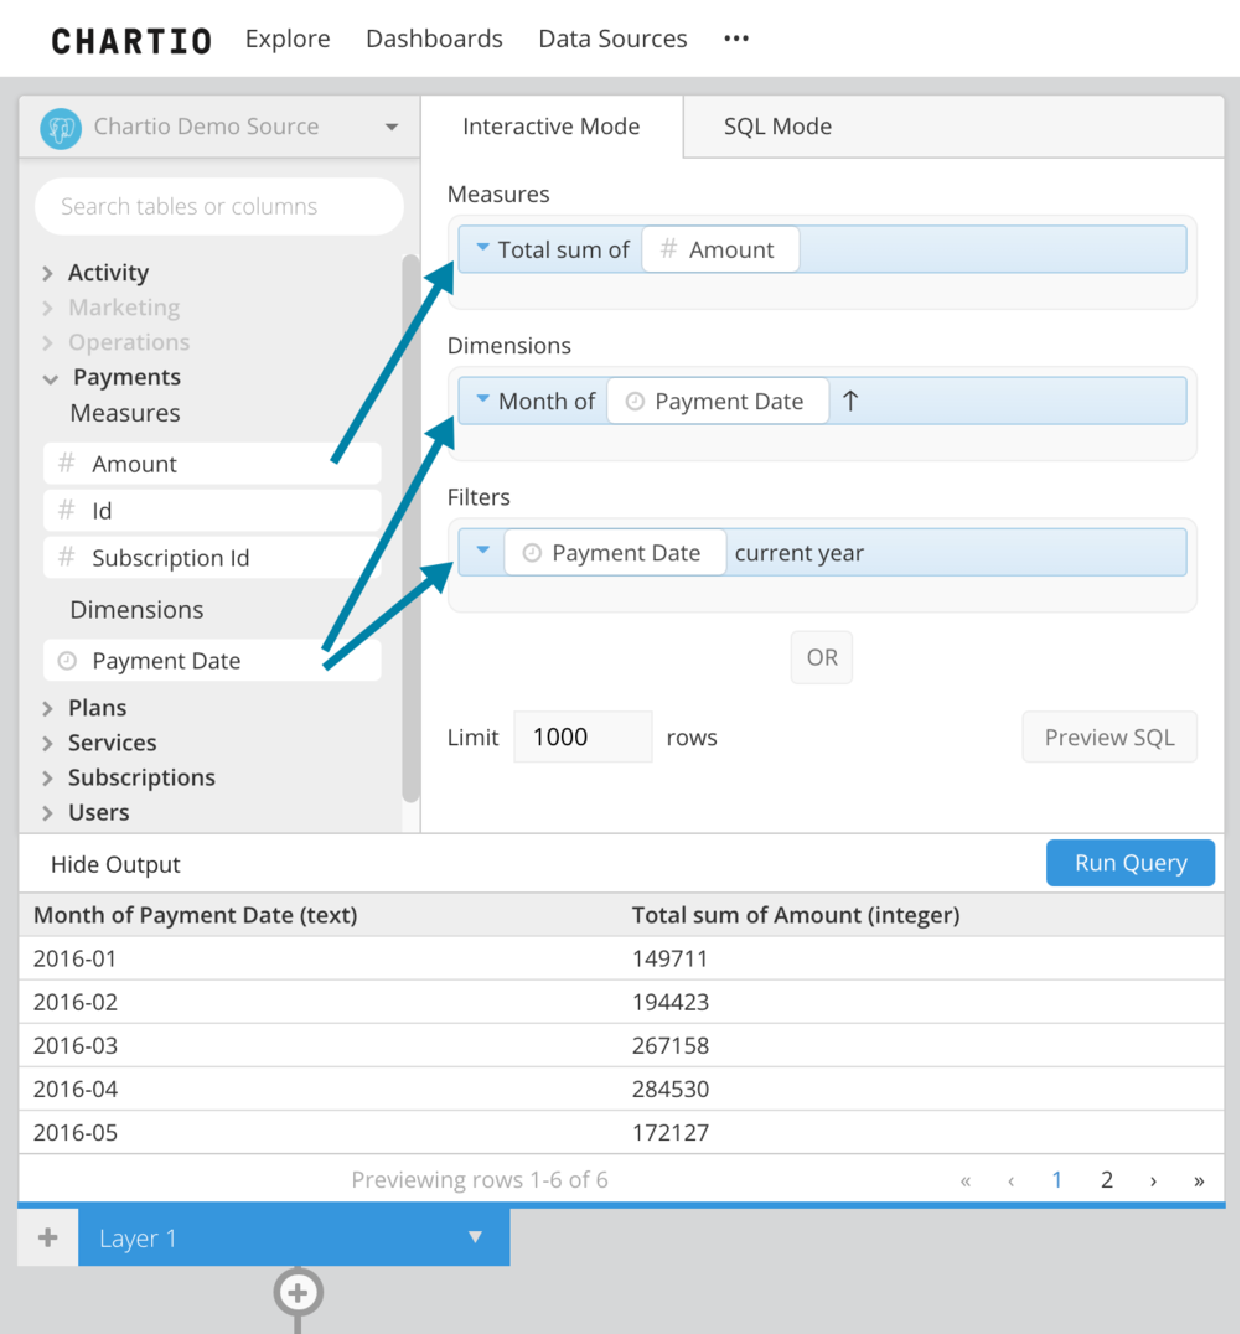
\includegraphics[width=0.5\linewidth]{chartio-data-explorer-data-source}}%
    \subcaptionbox{Chartio Visual SQL\label{fig:chartioVisualSQL} \cite{chartioVisualSQL}}%
      {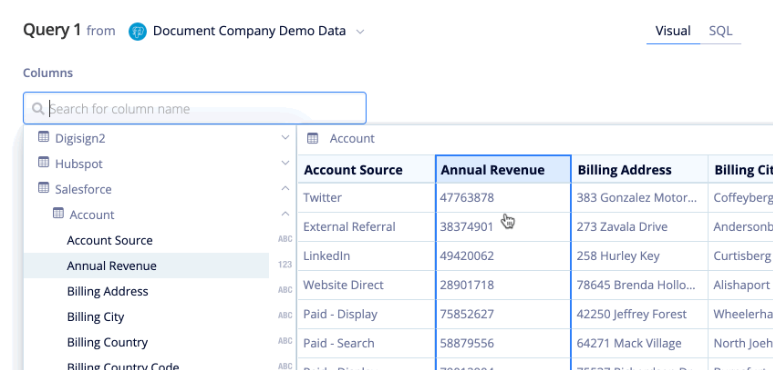
\includegraphics[width=0.5\linewidth]{chartio-visual-sql-data-source}}%
      \\
    \subcaptionbox{Tableau Prep\label{fig:tableauPrep} \cite{tableauPrepHelpWhatsNew}}%
    {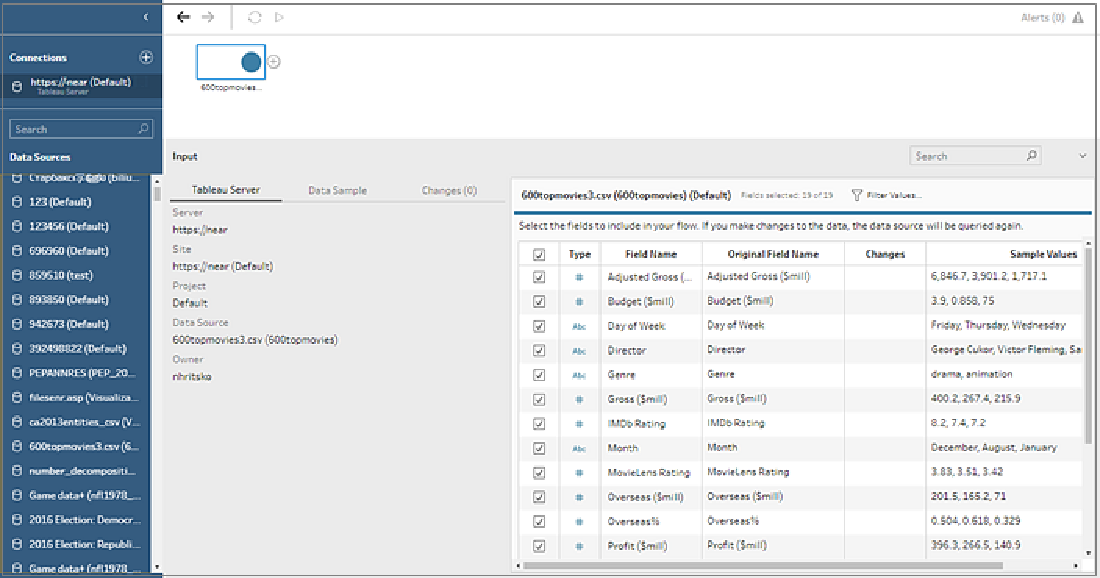
\includegraphics[width=0.5\linewidth]{tableau-data-source}}%
  \subcaptionbox{Devart dbForge Query Builder\label{fig:devartDbForge} \cite{dbForgeQueryBuilder}}%
    {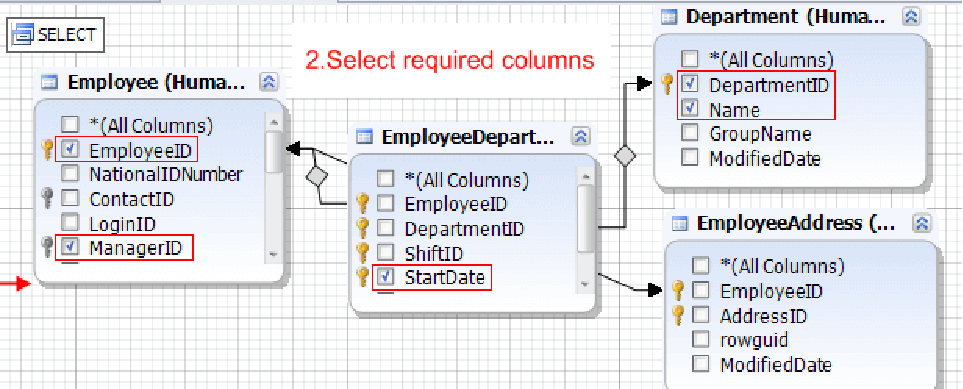
\includegraphics[width=0.5\linewidth]{dbforge-data-source}}%
  \caption{Different approaches to select the entities of the query.}
    \label{fig:approaches_select_data_sources}
  \end{figure}

  \bigskip

\textbf{Merge Type:}



Merges are used when it is necessary to extract data from different tables, so it is necessary to establish what is the join kind to merge the data. Therefore, the interface needs to adopt an interaction and representation technique to specify it. To define a join in Devart dbForge Query Builder \cite{dbForgeQueryBuilder}, the user can only select the attributes’ checkboxes of the different tables and the system generates an inner join automatically. In this system, there are buttons on the toolbar to select all rows of one table, of another, or both, allowing to perform left, right and outer joins respectively \cite{dbForgeMakingJoinsBetweenTables}.
  
Another approach used by some systems, such as Chartio Data Explorer \cite{chartioDataExplorer} and Microsoft Power BI \cite{powerBI}, is a form-based interface to insert a join. In the former, two queries can be merged clicking on a button to popup a form which can be used to select the merge type and the first columns that will be merged using dropdowns \cite{chartioDataExplorer} (Figure \ref{fig:chartioDataExplorerJoin}). Also, if there are null values on the merge related columns, there is an option to include or not the null values match rows \cite{chartioJoiningDataAcrossDatabases}. Similarly, the latter provides a button to merge queries that opens a modal where can be chosen the attributes that will be used on the merge (viewing also a table preview) and the join kind, using a dropdown \cite{powerBIShapeAndCombineData} (Figure \ref{fig:powerBIJoin}).
  
Tableau Prep \cite{tableauPrep} provides two options to start a join between two tables: clicking on a "add join" hover button above the table visual representation with suggestion of related tables, or merge the visual representation of two tables using a drag and drop action. After this selection, the inner join type is selected automatically by the system according to the tables relationship. \cite{tableauAggregateJoinOrUnionData} \cite{tableauAddMoreDataInTheInputStep} However, the user can configure the join in a dedicated section (Figure \ref{fig:tableauJoinPanel}) where it is possible to define the join type using a Venn Diagram, to manage the join clauses using dropdown lists to select the fields, including also some join clause recommendations based on the database schema. Moreover, a summary of the join result that contains counters with the values included and excluded by each table, in a visual way using diagrams is provided. Finally, there is presented a list of the values included and excluded, where the red values represent the values excluded, as well as a preview of the join result \cite{tableauAggregateJoinOrUnionData}.

\begin{figure}[htbp]
    \centering
    \subcaptionbox{Chartio Data Explorer\label{fig:chartioDataExplorerJoin} \cite{chartioDataExplorer}}%
      {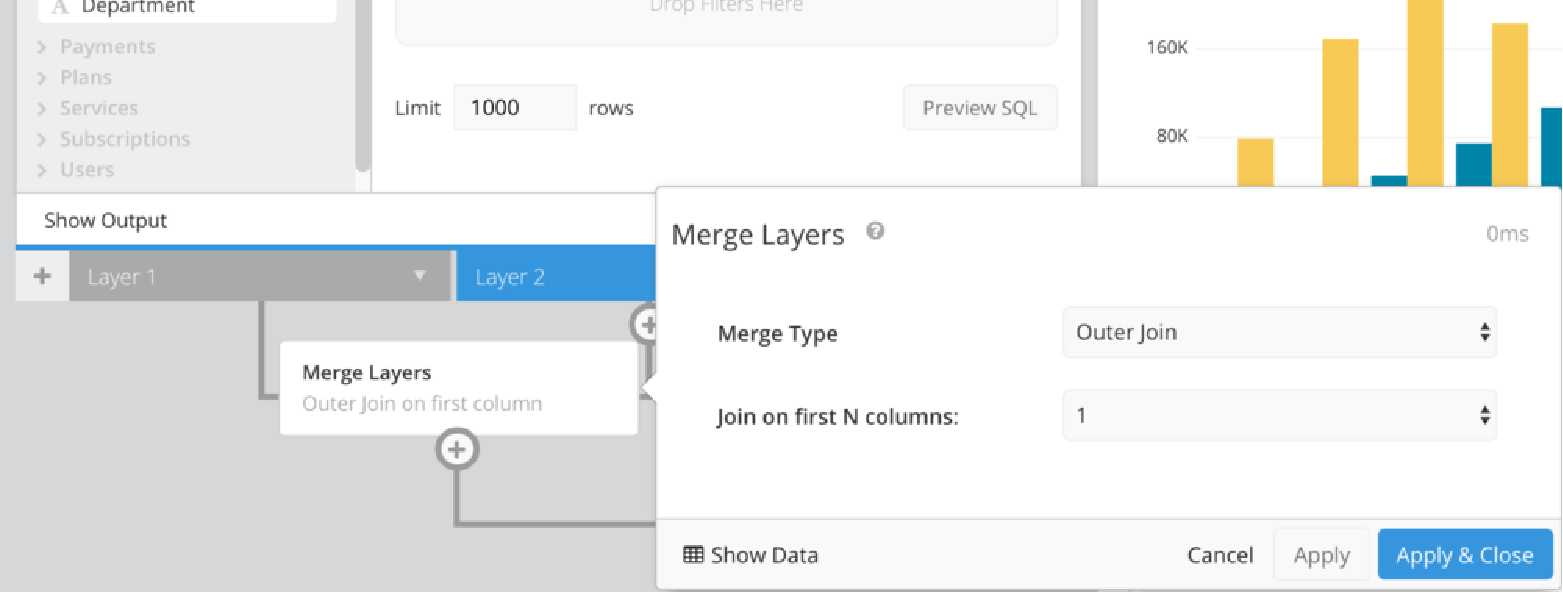
\includegraphics[width=0.4\linewidth]{chartio-data-explorer-join}}%
    \subcaptionbox{Microsoft Power BI\label{fig:powerBIJoin} \cite{powerBIShapeAndCombineData}}%
    {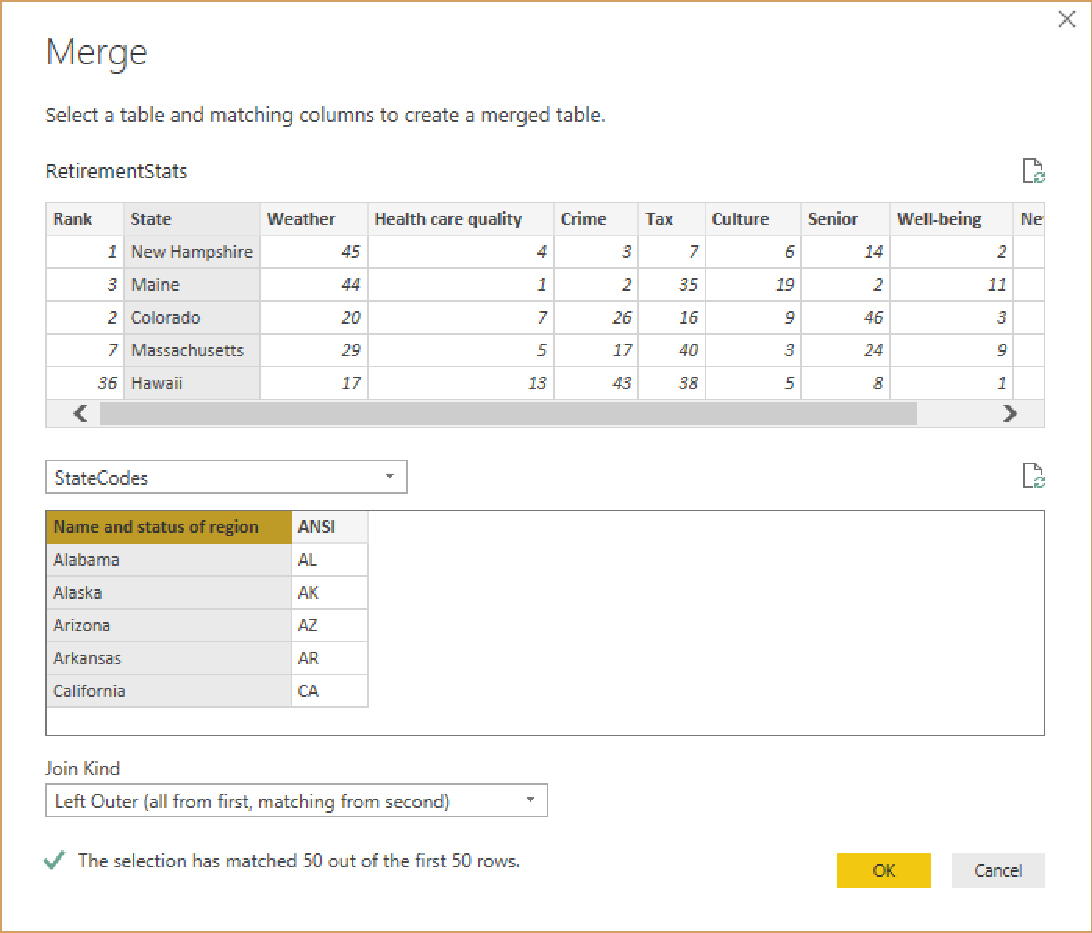
\includegraphics[width=0.4\linewidth]{power-bi-join}}%
    \\
    \subcaptionbox{Tableau Prep\label{fig:tableauJoinPanel} \cite{tableauAggregateJoinOrUnionData}}%
      {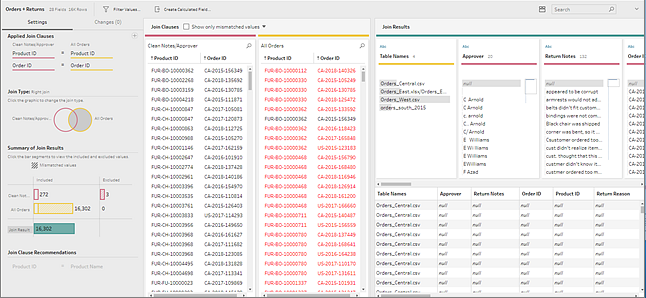
\includegraphics[width=0.8\linewidth]{tableau-join-panel}}%
  \caption{Data merging approaches.}
    \label{fig:approaches_select_data_sources}
\end{figure}

\bigskip

\textbf{Filtering Criteria}: 

To represent and manage the filtering criteria of the queries, usually is used text to indicate the logical conditions. However, some systems are trying to optimize the usability, helping the user in the specification process through some autocompletes. These diminish the necessity to remember all the syntax and the name of the functions. 
Besides, other systems present the logical conditions using a more structured layout, although keeping resorting in a textual representation. An example is Devart dbForge Query Builder \cite{dbForgeQueryBuilder} that represents the WHERE and HAVING clauses in a tree where the user can organize the conditions into groups \cite{dbForgeBuildingWhereOrHavingClause}.

Furthermore, some query systems also allow the user to view the query result, providing a shortcut in the column's name to insert filters. So, the user can change the query while is viewing the results. In this way, the user can apply a filter and view its effect almost immediately. Power BI Query Editor \cite{powerBI} is an example of a system which uses this approach.

Different interfaces can be used to select filters regarding the field data type. The advantages of the graphical interfaces could support the filtering criteria definition. For example, if a filter is applied to constraint dates, then a date input box with a visual calendar can be useful to simplify the date typing. In this way, some softwares, such as Chartio Visual SQL \cite{chartioVisualSQL} and Chartio Data Explorer \cite{chartioDataExplorer}, not only helps in the data typing, but also provide dropdown lists that contain operators that can be applied to the referred data type (e.g. less than, contains, like, etc)  to helps the user in the boolean operator specification \cite{chartioDataExplorer}  \cite{visualSqlActions}.

Tableau Prep \cite{tableauPrep} follows this in a more strict way, distinguishing between data types when filtering criteria are indicated. It provides different forms depending on the data type. The main difference of this system is that not only provides a more diversity of controls, as integrating range selectors, radio button, and the option to include or exclude fields through an action accessible near its value, but also gives to the user to option to use a calculation form where the interaction style is more textually and more extensible \cite{tableauFilterYourData}.

\bigskip

\textbf{Sorting Criteria}: 

\bigskip

\textbf{Aggregation Functions}: 

\bigskip

\textbf{Other Specifications}: 


\section{Discussion}
\label{sec:discussion}